\chapter{Spatial Analysis}
Many of the methods introduced in this thesis will rely on works developed in the fields of Spatial Statistics, Geostatistics, and Geography. Geo-statisticians have developed much of the work surrounding field predictions in the geospatial domain. The Kriging Method, a best linear unbiased predictor (BLUP) produces a prediction based on statistical data gathered from samples taken on a field. The Kriging Method predicts the state of a point on a field from weights generated from a covariance matrix created from samples on the field. A variance for each computed prediction can also be generated as a byproduct of the Kriging prediction, and this will be used to calculate information gain in the path finders introduced in this paper. It is assumed that the expected value of each point is from a normal distribution, where the variance and expected value of the distribution is a function of the neighboring samples and spatial autocorrelation factor of the field.

Tobler's First Law of Geography \cite{tobler:first_law} states,``Everything is related to everything else, but near things are more related than distant things." Regarding geospatial data, there is a positive correlation between observations with a small difference in distance \cite{miller:on_toblers_first_law}. This implies the existence of geospatial autocorrelation in many target fields of interest, where there exists a positive correlation between elements in a field. Geospatial autocorrelation is the hypothesis that allows naive prediction techniques, like Inverse Distance Weighting (IDW) (Section \ref{sec:idw_intro}), to work. The Kriging Method first finds the underlying spatial autocorrelation of a target field from a set of samples, and then predicts the state of a given vesicle by emphasizing values of statistically similar samples in a weighted sum. The methods introduced in this chapter are intended to serve as an introduction and background into the Kriging Method.

\subsection{Autocorrelation in a Field}
Positively correlated spatial autocorrelation in a field implies the existence of a cluster of similar points near one another i.e. relatively small covariances between two spatially similar points. The opposite is true when the overall spatial autocorrelation of a field is negative. Using Tobler's First Law of Geography, the assumption that fields measured will contain positive autocorrelation will be used. The degree of spatial autocorrelation in a field can be measured, and will be discussed in Section \ref{sec:vario} on Variography.

\begin{figure}[ht!]
    \centering
    \begin{subfigure}[t]{0.5\textwidth}
        \centering
        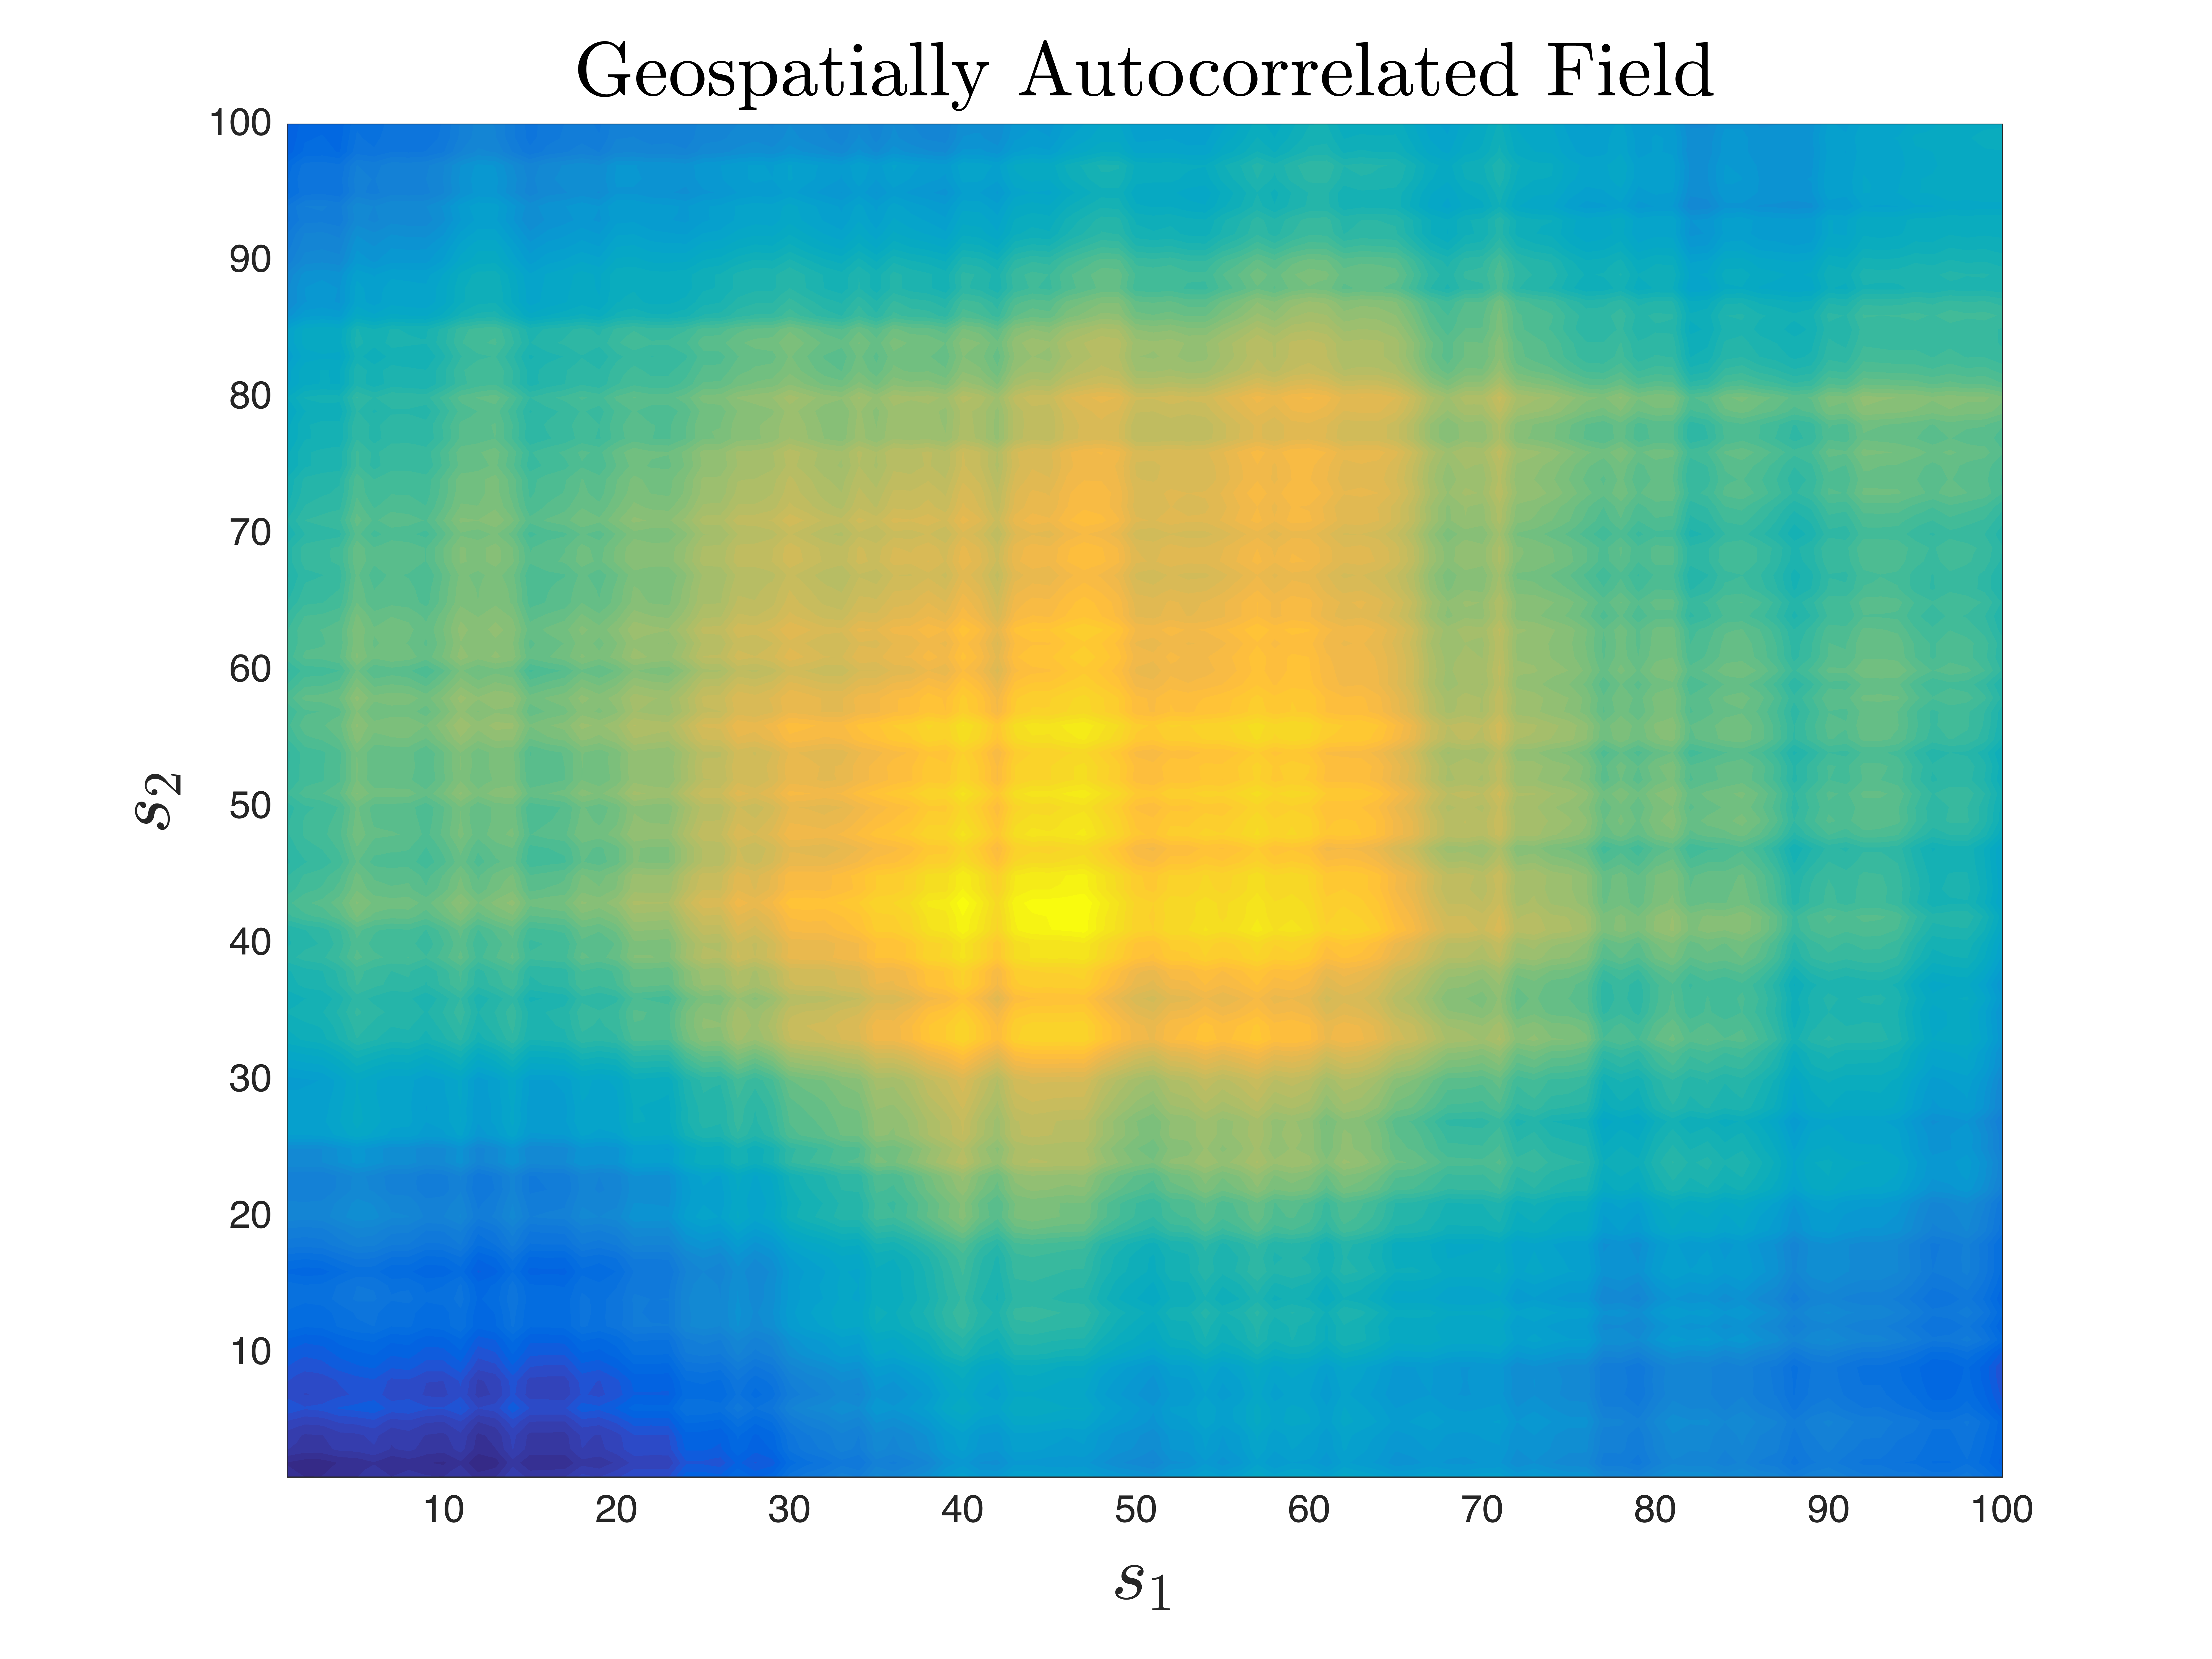
\includegraphics[width=\linewidth]{figures/generated_field.png}
        \captionsetup{skip=0.5\baselineskip,size=footnotesize}
        \ssp
        \caption{A randomly generated spatially autocorrelated field.}
		\label{fig:gen_field}
    \end{subfigure}%
    ~ 
    \begin{subfigure}[t]{0.5\textwidth}
        \centering
        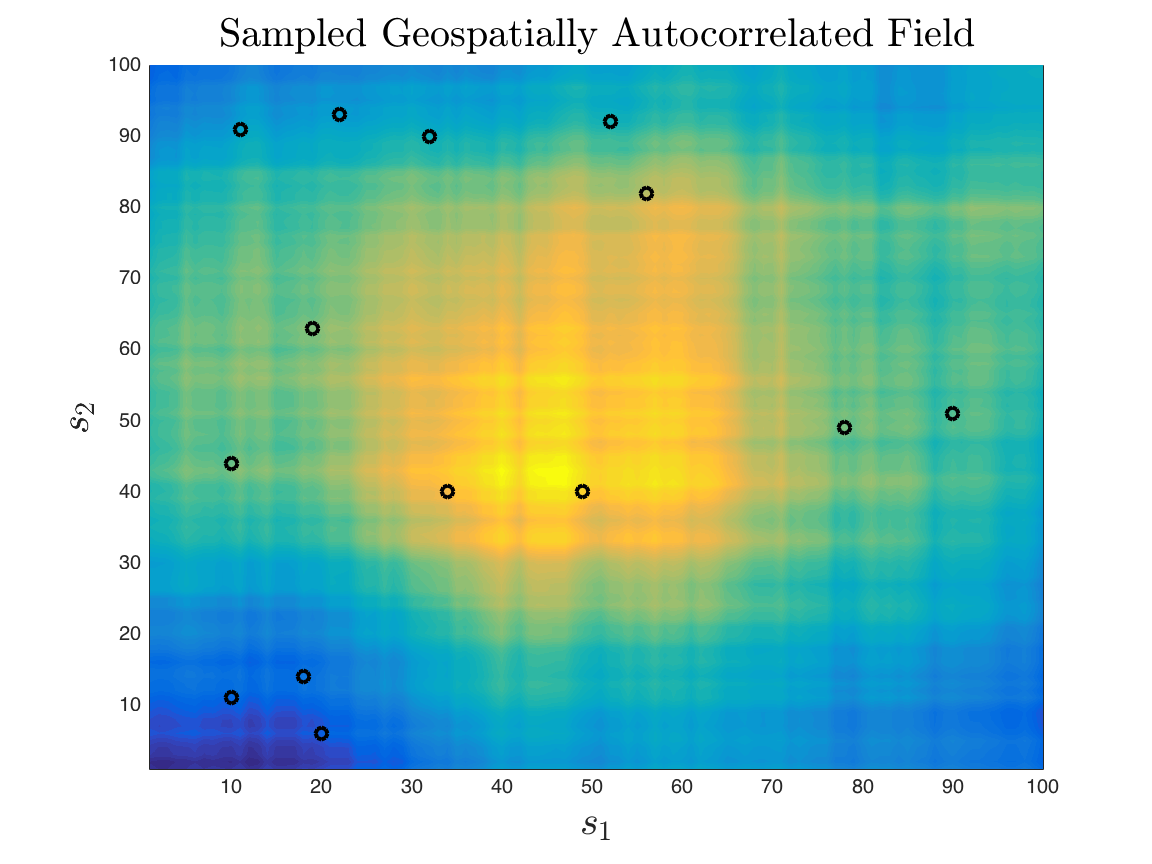
\includegraphics[width=\linewidth]{figures/sampled_generated_field.png}
		\captionsetup{skip=0.5\baselineskip,size=footnotesize}
		\ssp
        \caption{Samples at marked locations were taken of the target field in \ref{fig:gen_field}.}
		\label{fig:sampled_field}
    \end{subfigure}
    \ssp
    \caption{A Gaussian distributed randomly generated spatially autocorrelated field.}
    \label{fig:generated_and_sampled_field}
\end{figure}

\section{Inverse Distance Weighting} \label{sec:idw_intro}
An inverse distance weighting is a naive interpolation tool where a point is predicted based its distances from a set of observed points. A simple IDW, using Shepard's Method \cite{shepard:idw}, gives a prediction, $\hat{Z}(\vect{s}_j)$, of an unobserved point, $\vect{s}_j$, as a function of the $N \in \mathbb{N}$ observed points, $\{Z(\vect{s}_1), Z(\vect{s}_2), \hdots, Z(\vect{s}_n) \}$.

\begin{equation}
	\hat{Z}(\vect{s}_j)=\begin{cases}
			\dfrac{\sum\limits_{i=1}^N [w(\vect{s}_j, \vect{s}_i)] Z(\vect{s}_i) }{\sum\limits_{i=1}^{N} w(\vect{s}_j, \vect{s}_i)} & \text{if}\ \forall i \mid d(\vect{s}_j,\vect{s}_i) \neq 0\ \\
			Z(\vect{s}_j) & \text{if}\ \exists i \mid d(\vect{s}_j,\vect{s}_i)=0\\
		\end{cases}
\end{equation}
\begin{equation}
    d(\vect{s}_j,\vect{s}_{i})=\|\vect{s}_j-\vect{s}_i\|_{2}
\end{equation}
\begin{equation}
	w(\vect{s}_j, \vect{s}_i)=\frac{1}{d(\vect{s}_j,\vect{s}_{i})^{p}}=\|\vect{s}_j-\vect{s}_i\|_{2}^{-p}
\end{equation}

\noindent where $p \in \mathbb{R}^{+}$ is the IDW "power parameter". The power parameter, $p$, controls the emphasis on near and far observations on a prediction. As $p$ increases, the predicted values more closely resemble the closest made observation to the prediction location. Inversely, as $p$ gets smaller within $(0, 1]$, more emphasis is drawn from observations made further away.\\

\begin{figure}[ht!]
    \centering
    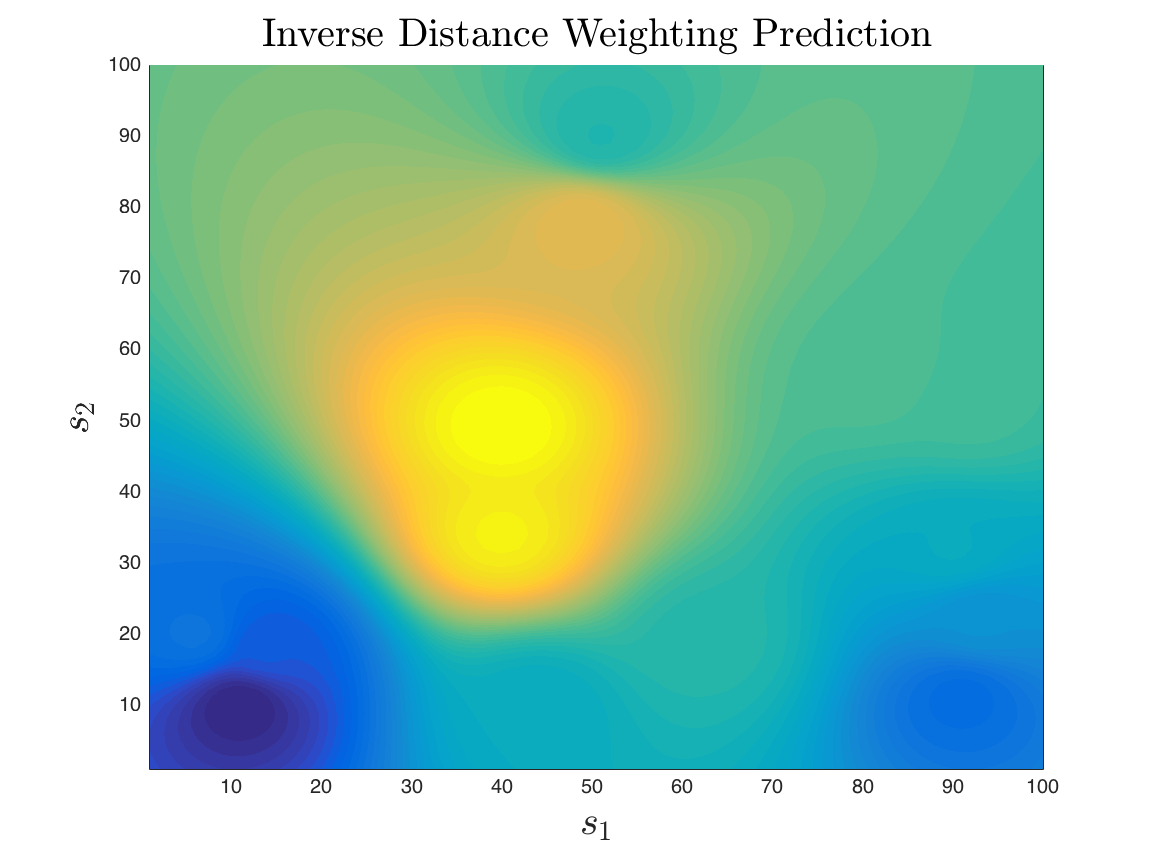
\includegraphics[width=0.8\linewidth]{figures/idw_predicted_field.png}
    \ssp
    \caption{An inverse distance weighting predicted field generated from the samples taken of Figure \ref{fig:gen_field} at the locations marked in Figure \ref{fig:sampled_field}.}
    \label{fig:idw_field}
\end{figure}

This method can yield a prediction for all possible points in a field where a set of observations at known locations are made, as done in Figure \ref{fig:idw_field}. Unfortunately, the method is limited in that it assumes a spherical distribution of correlation of points in a field, and does not take advantage of the underlying spatial correlation patterns of the target field being observed to make a more methodical weighted sum prediction. A field that exhibits properties of spatial autocorrelation would be more statistically exploitable because the distribution of the states of interest on the field can be learned.

\section{Variography} \label{sec:vario}
Variography is a set of procedures for examining and interpreting spatial dependence and spatial autocorrelation in a field of observed data. The \textit{variogram} of a field will be introduced to assist in extracting the underlying spatial autocorrelation function of a target field. The variogram function will be factored into a classical prediction via weighting, yielding a Kriging Weighting.

\subsection{The Variogram}
A variogram quantifies dependence for two disjoint observations separated by some distance, or \textit{lag}, away. The function, in essence, yields a value directly proportional to the covariance between two given points in a stochastic field.

A Variogram is intended to be a continuous function which yields a covariance between two points $Z(\vect{s}_{i})$, $Z(\vect{s}_{j})$, which have not necessarily been observed, but known to be a Euclidean distance, or lag, $h_{i,j} \in \mathbb{R}$ apart \cite{deutsch:geostat}, where

\begin{equation}
h_{i,j} = \| \vect{s}_i - \vect{s}_j \|_2
\label{eq:hdist}
\end{equation}

Using the assumption on what a point's value on a field is constructed of is made in Equation 2.4.1 of Matheron, 1963 \cite{matheron:geostat}:

\begin{equation}
    Z(\vect{s}_i)=\mu(\vect{s}_i)+\theta(\vect{s}_i)
    \label{eq:matheron:assum}
\end{equation}

\noindent where $\theta(\cdot)$ is a zero-mean intrinsically stationary stochastic Wiener process, and $\mu(\cdot) = \bar{Z}$ is the mean value of the state of interest in the field.

\subsection{The Semivariogram}
The Semivariogram is defined to be the average squared difference between two points separated by some distance apart. Matheron, 1963 defines a semivariogram in \cite{matheron:geostat} in three-dimensional space as:

\begin{equation}
    \gamma(h) = \frac{1}{2A} \iint_A [ Z(\vect{s} + h) - Z(\vect{s}) ]^2 dA
    \label{eq:semivariogramint}
\end{equation}

\noindent where $A$ is a closed area in a field to consider, $Z(\vect{s})$ is the value of a point at location $\vect{s}$ on the field, and $Z(\vect{s} + h)$ is the value of some point a distance $h$, defined in Equation \ref{eq:hdist}, apart from a point $\vect{s}$ on the field.

It is infeasible to estimate an observation value at each possible point in the field to compute a continuous Semivariogram. Furthermore, the fields observed using these methods are typically gridded, and therefore not continuous by their analytical nature. A discrete model must first be constructed, and will then be fit into a continuous variogram model. This is done by first constructing a discrete variogram model, or \textit{Empirical Semivariogram}, and then fitting a continuous model to it. Fitting a discrete Semivariogram should in turn yield a function close to $\gamma(h)$ defined in Equation \ref{eq:semivariogramint}, and should be identical given that every point in the area $A$ is sampled with infinite precision.

\subsection{The Empirical Semivariogram}
An Empirical Semivariogram, or Experimental Semivariogram, is a discrete function representing the covariance of the observation value difference between two sampled locations that are some distance $h$ apart. Goovaerts defines the empirical variogram in \textit{Geostatistics for Natural Resources Evaluation. Applied Geostatistics Series} \cite{goov:97} as:

\begin{equation}
    \label{eq:exp_var}
    \hat{\gamma}(h) = \frac{1}{2N(h)}\sum_{i=1}^{N(h)} (Z(\vect{s}_i) - Z(\vect{s}_i+h))^2
\end{equation}

\noindent where $N(h)$ is the cardinality of the set of all pairs of observed points that are a Euclidean distance, or lag, $h$, apart.

The experimental variogram conveys the spatial autocorrelation of a sampled field. As the lag between two given points increases, the covariance also increases when the field is spatially autocorrelated. The covariance levels out to a steady value (the \textit{sill}) at some distance in the domain (the \textit{range}). The range marks the point where the loss of reliable spatial autocorrelation between two points ceases.

\begin{figure}[ht!]
    \centering    
    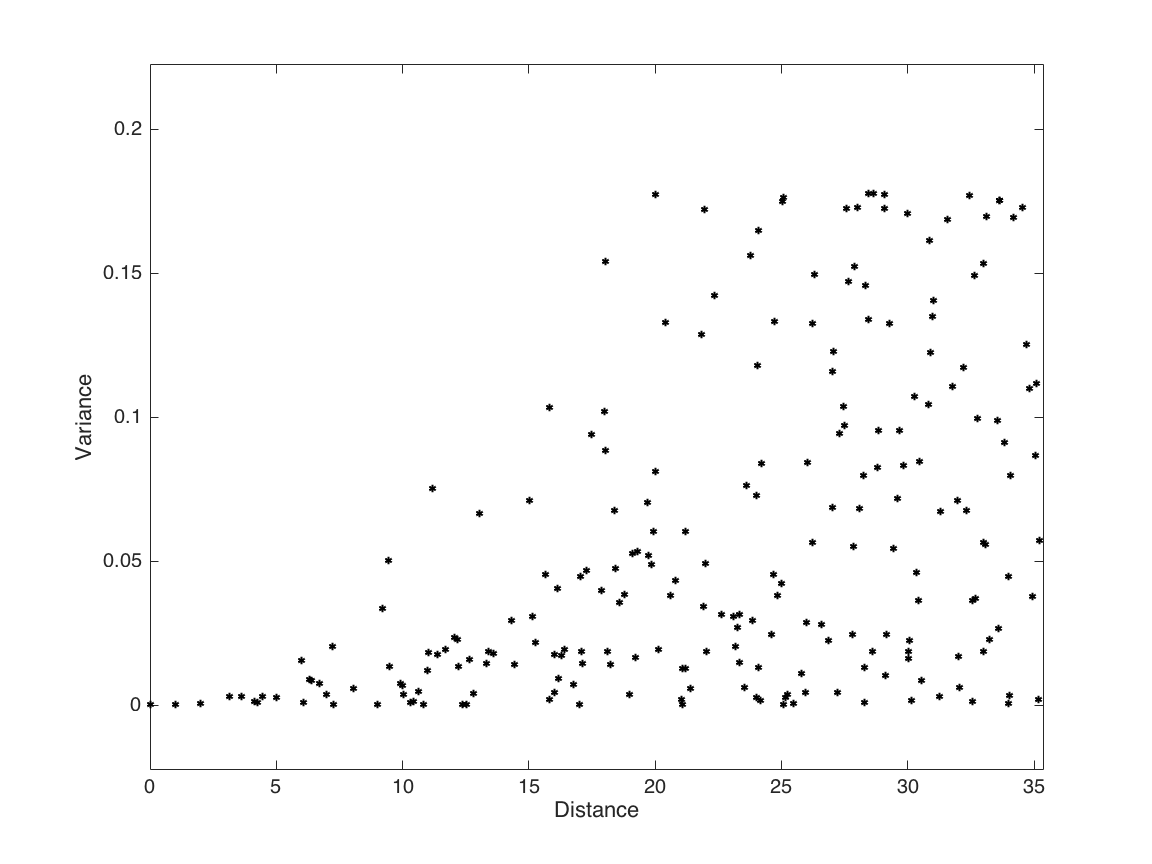
\includegraphics[width=0.8\linewidth]{figures/exp_variogram.png}
    \ssp
    \caption{An empirical semivariogram.}
    \label{fig:emp_semiv}
\end{figure}

\subsection{Converting a Semivariogram to a Variogram} \label{sec:semitovar}
The intent of fitting a statistical model to an experimental variogram is to approximate the continuous covariance for any two points, that have not necessarily been observed, on $Z$ that are at some known lag apart.

\subsection{Variogram Models} \label{sec:variomodels}
The Empirical Semivariogram will be fit to a statistical model, or \textit{kernel}, known as a Variogram Model. There exist some well known models, further discussed in this section. Each model is a scalar function of lag, $h$, \text{sill}, $s$, and \text{range}, $a$. The term \textit{sill} refers to the point on the co-domain where two points at the lag specified are no longer autocorrelated. The sill is therefore the largest value of covariance for two disjoint points on a field that are still considered to be autocorrelated. The corresponding point on the domain for the sill is referred to as the \textit{range} on the variogram. Two points that have a lag larger than the range are not considered to be autocorrelated.

The \textit{nugget} of the variogram is defined to be the variance at zero separation, or $\gamma(0)$ \cite{matheron:geostat}. This value is exactly zero for ideal measurements, but is generally not for real-life measurements. The value found for the nugget is typically summed with the value yielded by $\gamma$, to get the final variogram value for a given lag \cite{goov:97}.

\subsubsection{The Gaussian Model}

\begin{equation}
	\gamma_g(h, s, a) = s \Bigg[ 1 - \exp \Bigg( -\dfrac{h^2}{a^2} \Bigg) \Bigg]
	\label{eq:gauss_model}
\end{equation}

The Gaussian model will asymptotically reach its sill. The sill would be at the limit as $h$ approaches infinity. The \textit{practical range} is therefore used to refer the point on the domain where the variogram reaches 95\% of its sill \cite{goov:97}.

\subsubsection{The Exponential Model}

\begin{equation}
	\gamma_e(h, s, a) = s \Bigg[ 1 - \exp \Bigg( \dfrac{h}{a} \Bigg) \Bigg]
	\label{eq:exp_model}
\end{equation}

The same rules as the Gaussian model apply to the Exponential model \cite{goov:97}.

\subsubsection{The Spherical Model}

\begin{equation}
	\gamma_s(h, s, a) = \frac{s}{2} \Bigg[ \dfrac{3h}{a} - \Bigg( \dfrac{h}{a} \Bigg)^3 \Bigg]
	\label{eq:sph_model}
\end{equation}

The spherical model will reach an exactly zero slope at the sill and range \cite{goov:97}.

\begin{figure}[htb!]
    \centering    
    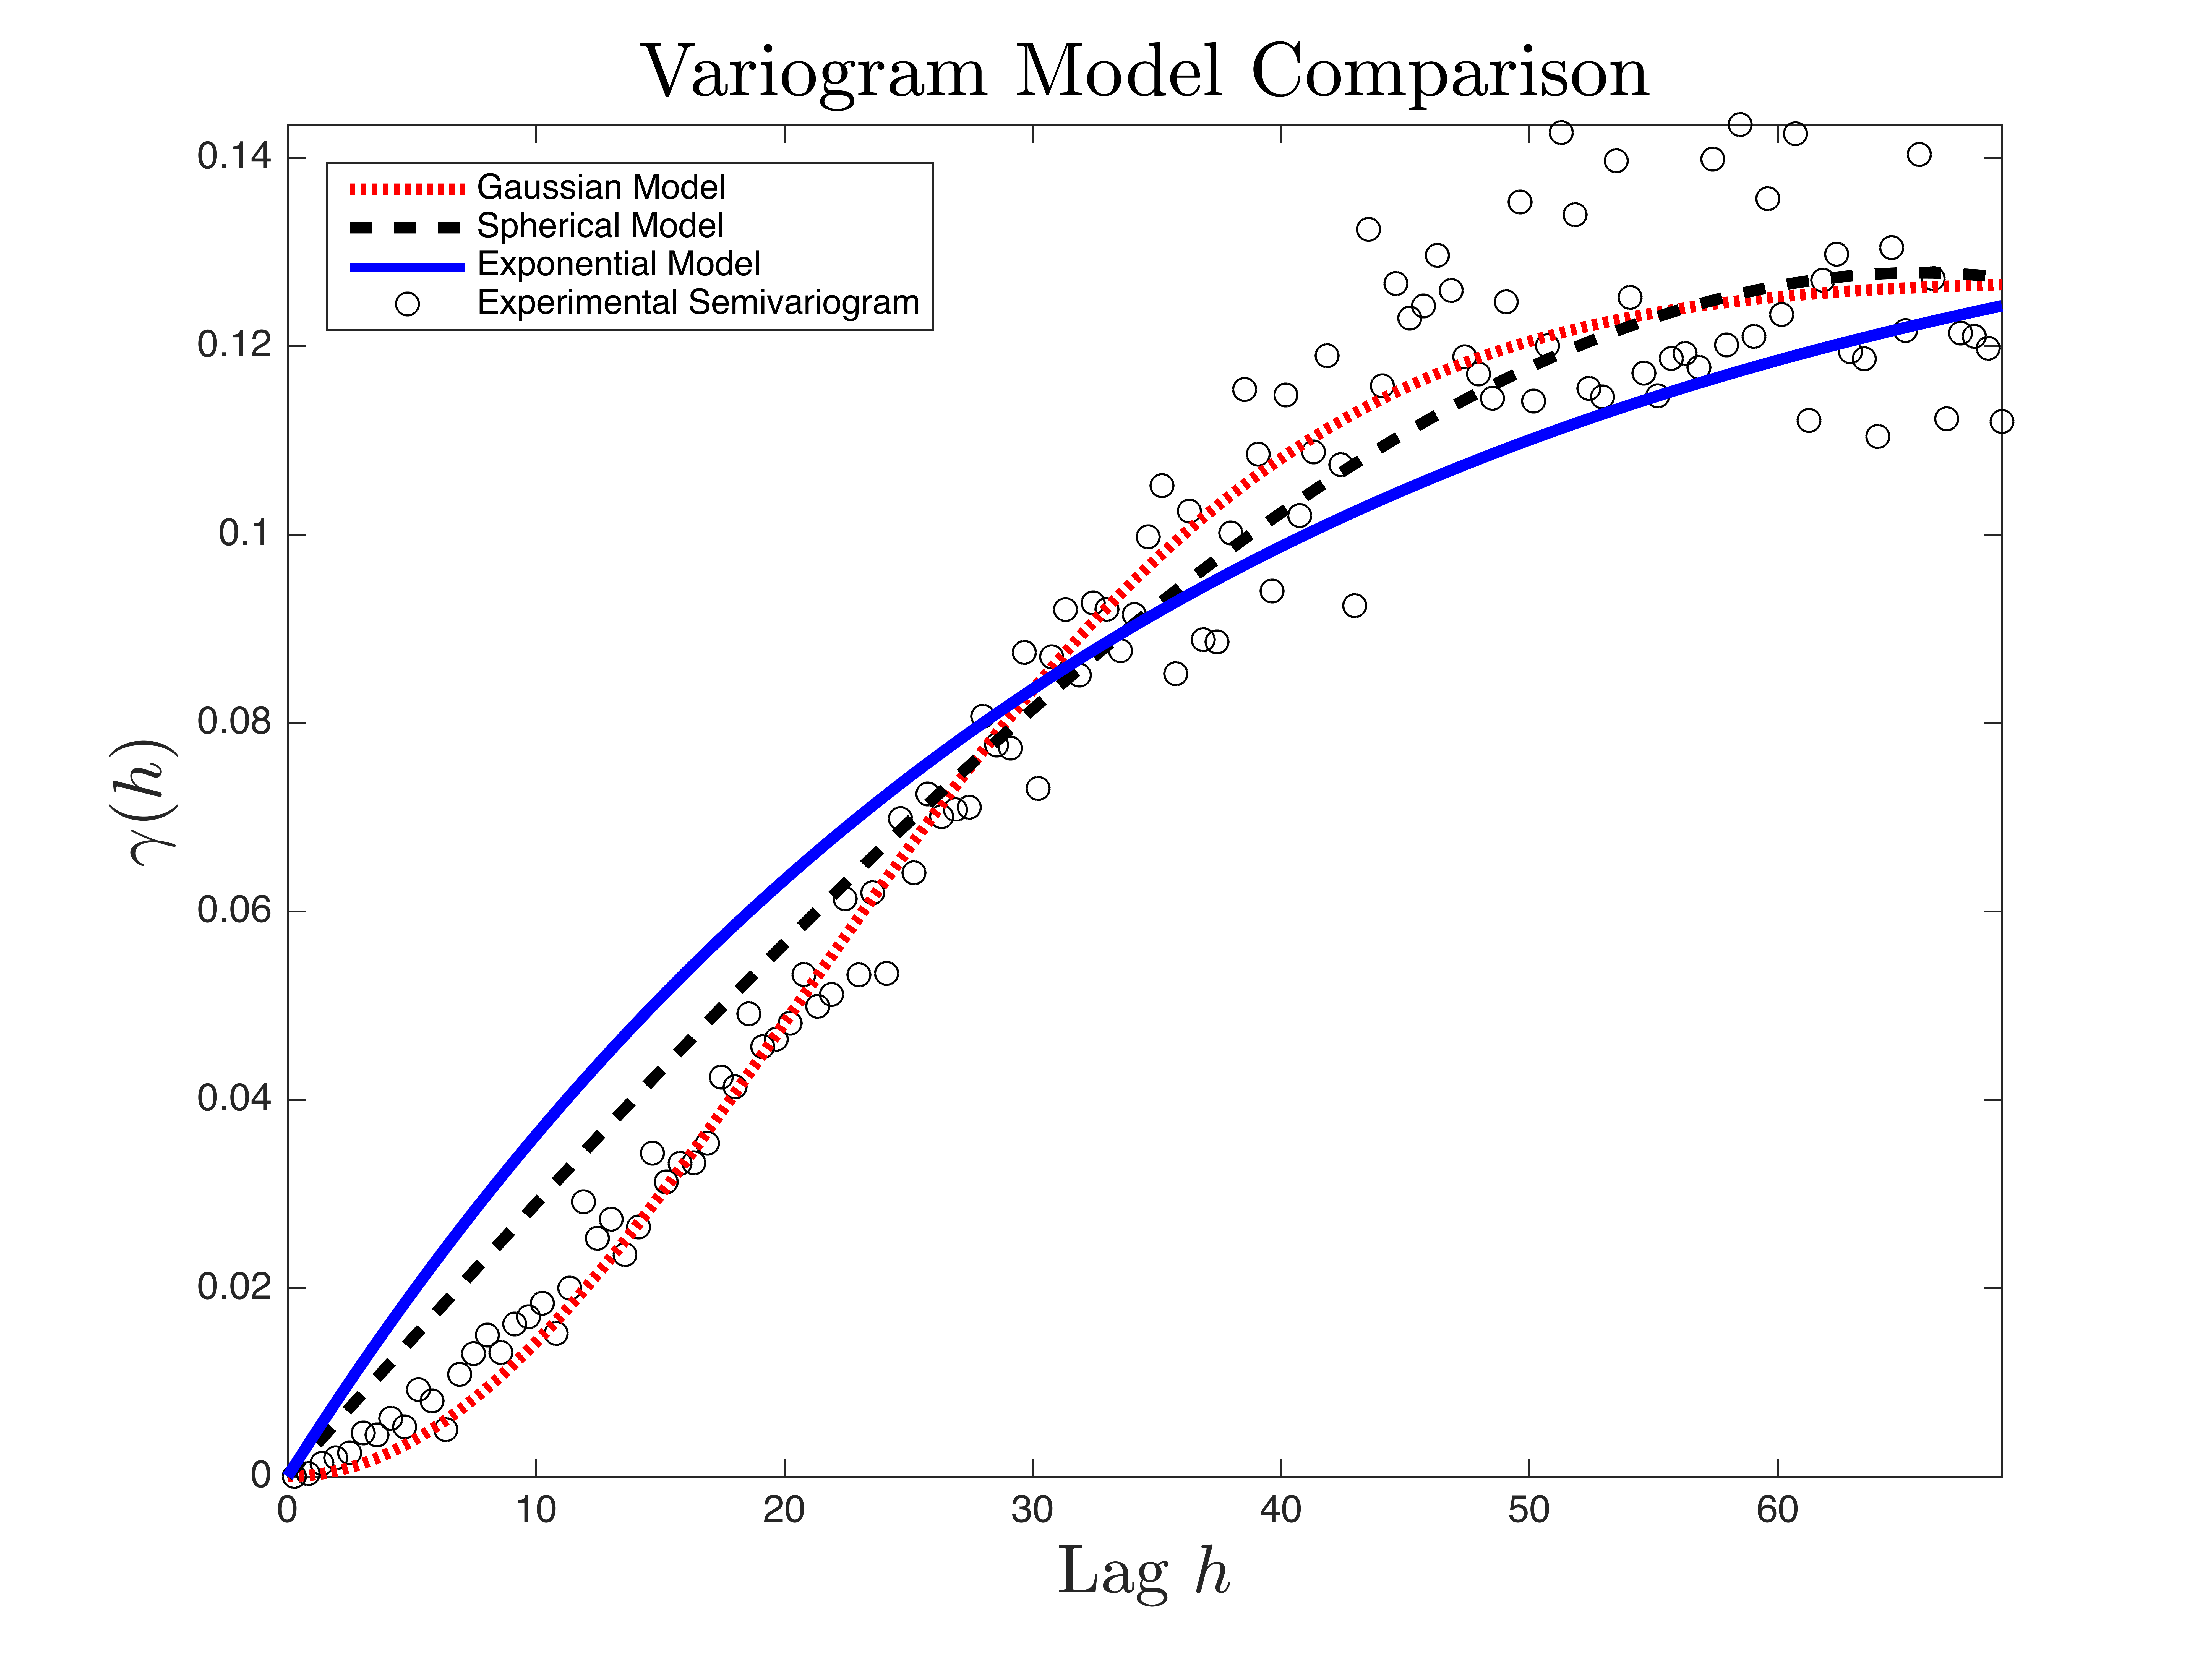
\includegraphics[width=0.8\linewidth]{figures/fit_kern_comp.png}
    \ssp
    \caption{Examples of three different variogram models.}
    \label{fig:fit_kernel_cop}
\end{figure}

\subsection{Fitting A Semi-Variogram} \label{sec:varfit}
The kernel function of the range, $a$, the sill, $s$, and lag, $h$ is chosen based on the statistical properties of the field being examined. Although there exist no closed form solution for finding an appropriate variogram model for a given field, one can compare a variety of different models against one another. Conducting cross-validation tests and comparing root-mean squared prediction errors for different models are common approaches for finding appropriate variogram models.

\subsubsection{Fitting a Variogram Using MATLAB}
Using a version of the \textit{fminsearch} function in \textit{MATLAB}, a variogram can be fit to the desired objective function from a set of samples and initial guesses for the range and sill using a simplex search method. As the function is used over several iterations of sampling, the fit range and sill values found in the previous iteration can be used as the seed to the next iteration of the fit in an attempt to minimize computation time. The \textit{MATLAB} function, \textit{fminsearch}, is defined to ``find the minimum of an unconstrained multi-variable function using a derivative-free method" \cite{mathworks:fminsearch}, expressed in Equation \ref{eq:matlabfmin}.

\begin{equation}
    \gamma(h) = \min\ [\gamma_{kernel}(h,s,a) - \hat{\gamma}(h)]^2
    \label{eq:matlabfmin}
\end{equation}

The function is then modified by specifying bounds of minimization in an attempt to decrease iterations of the function fit, which can be computationally expensive as more samples are taken. This modified version of \textit{fminsearch}, named \textit{fminsearchcon}, can be downloaded from the MathWorks File Exchange.

\begin{figure}[ht!]
    \centering    
	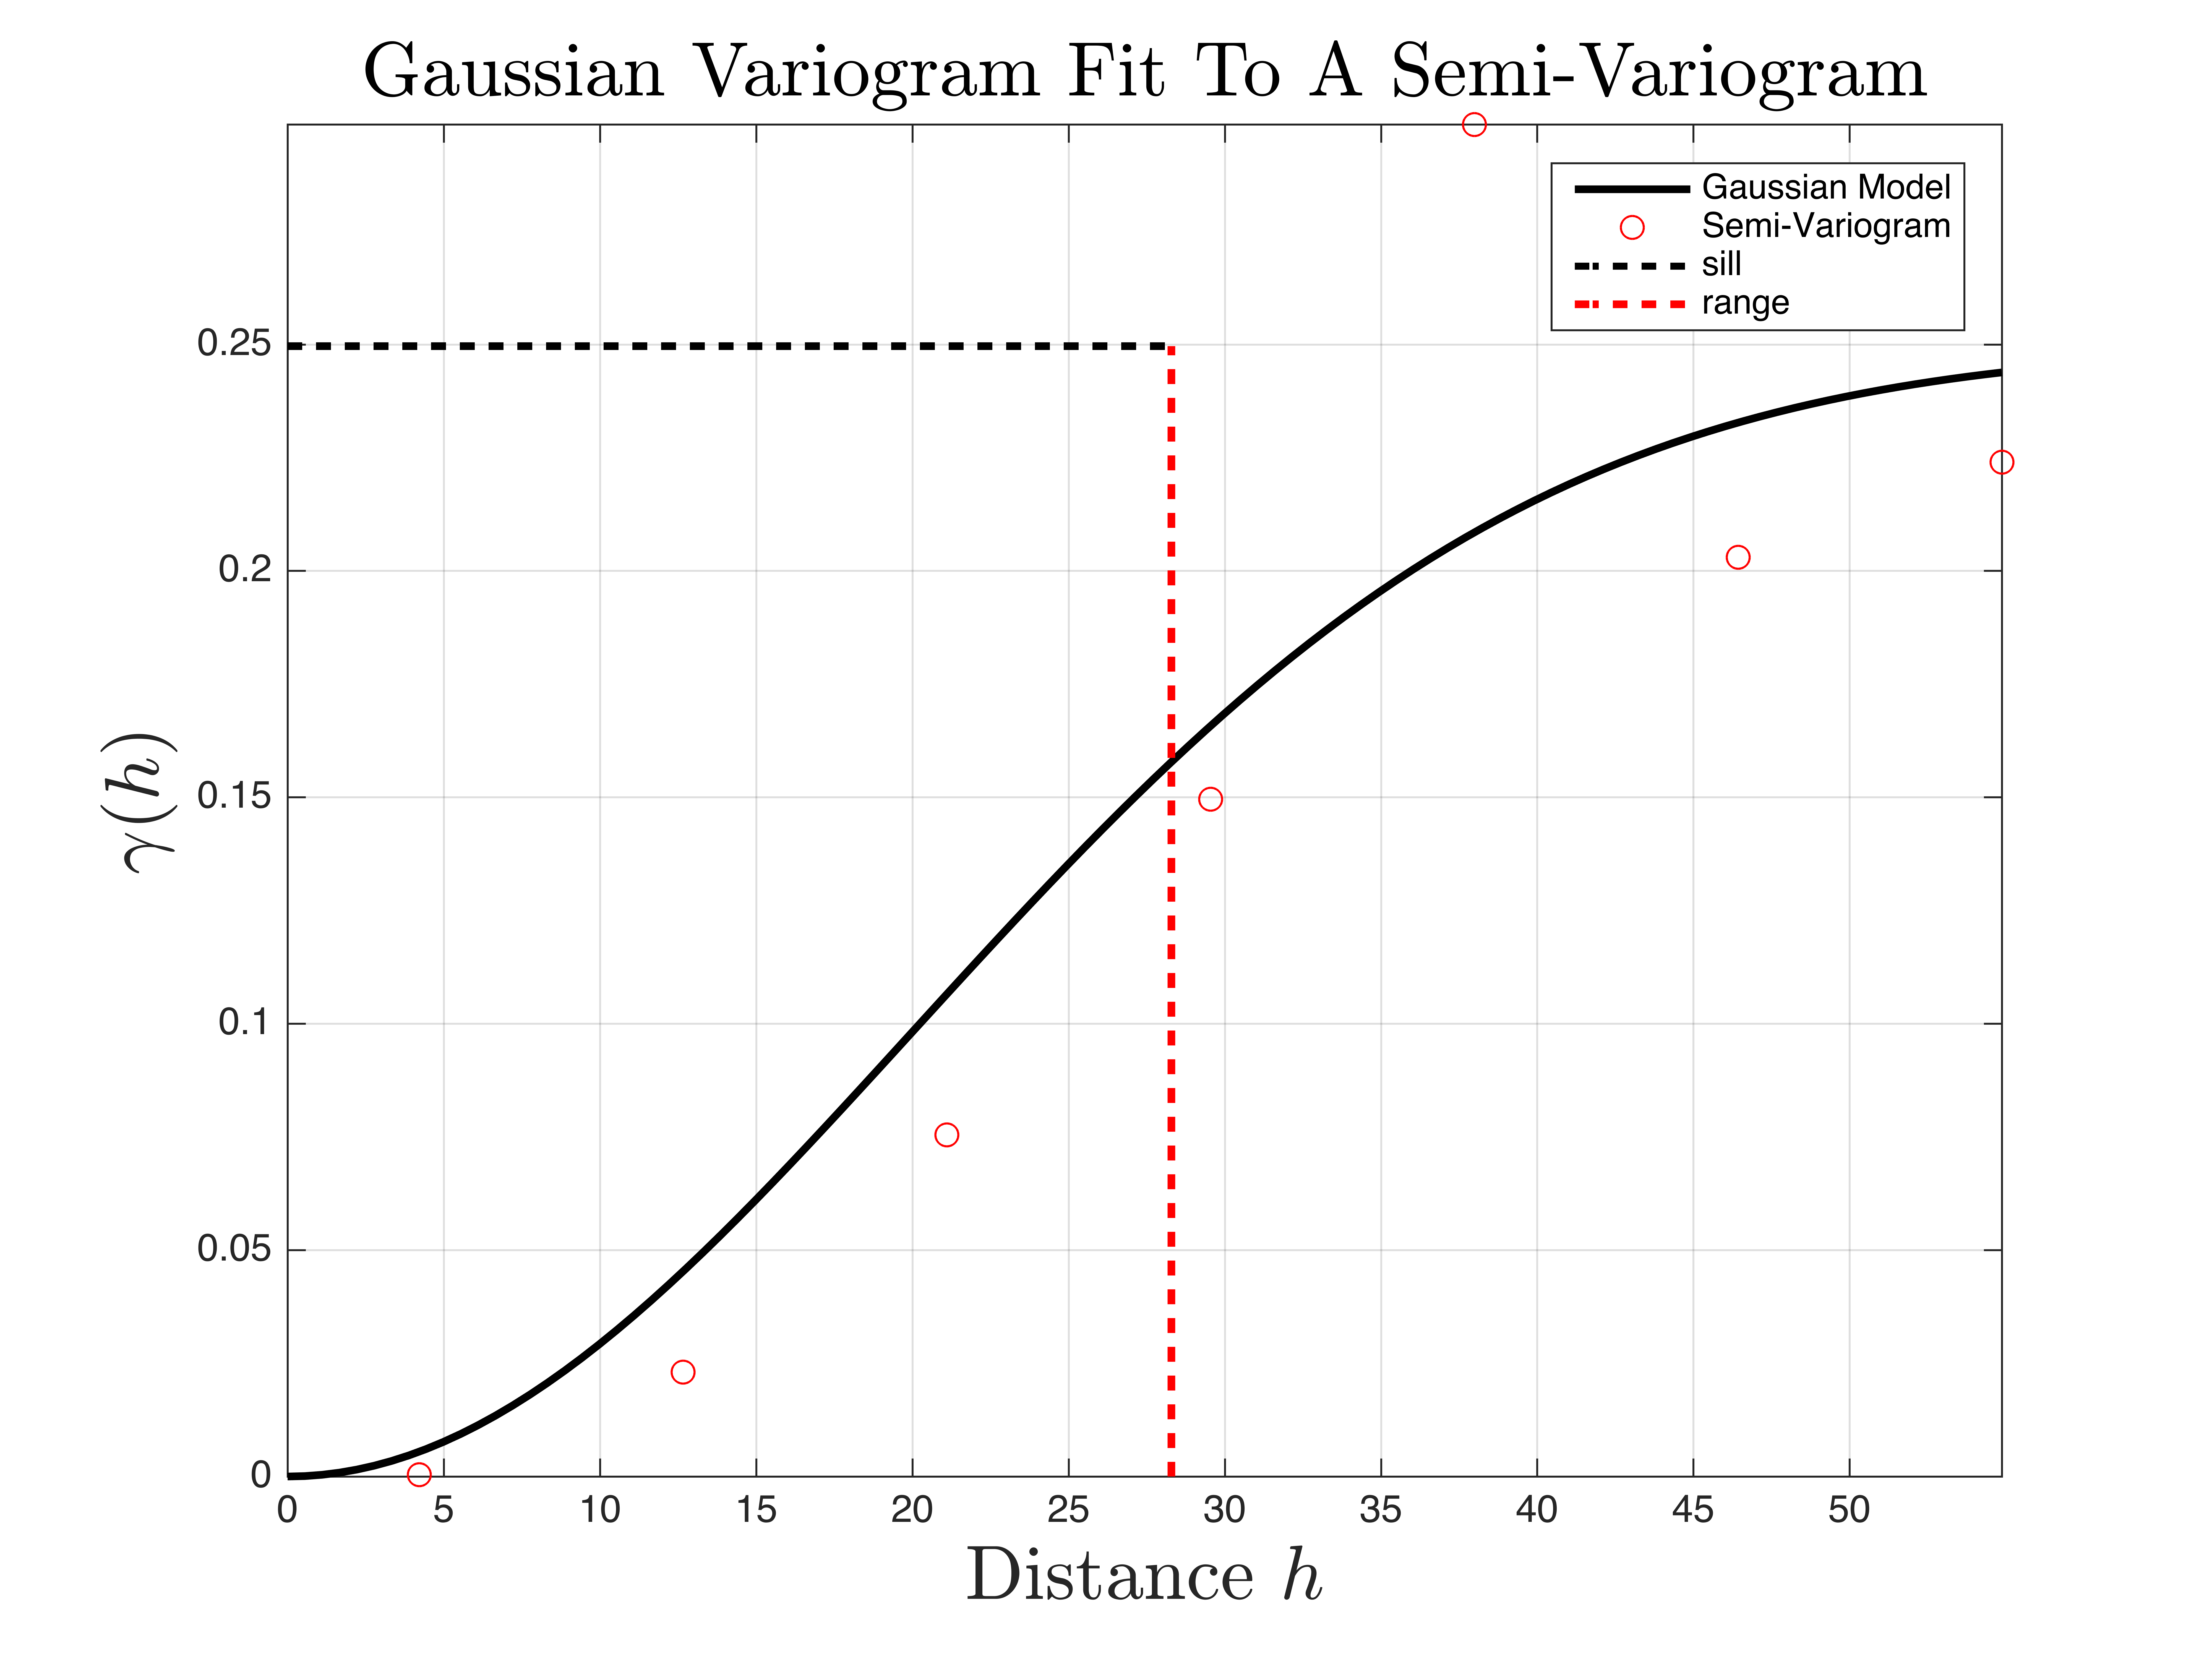
\includegraphics[width=0.8\linewidth]{figures/fit_kernel.png}
    \ssp
	\caption{An experimental variogram generated using Equation \ref{eq:exp_var} from the samples taken in Figure \ref{fig:sampled_field}. $\delta$ was chosen such that for $n$ observations, a total number of $\Big\lfloor \frac{n}{2} \Big\rfloor$ points were plotted. A Gaussian statistical model was fit to the experimental variogram. The variogram was fit using \textit{fminsearchcon} in \textit{MATLAB}.}
	\label{fig:fit_kernel}
\end{figure}

\section{The Kriging Method}
The Kriging Method conducts a weighted sum using the continuous variogram model that was fit to the physical observations made. The method can yield a prediction for each vesicle in a target space similar to the Inverse Distance Weighting method described in Section \ref{sec:idw_intro}, but with more statistical robustness.

\subsection{Forms of the Kriging Method}
There exist three major forms of the Kriging Method. All of which differ primarily in the handling of the mean gathered from observations of a target field. The \textit{Simple Kriging Method} makes the assumption that the mean is known and constant throughout the entirety of an observed field. This is of course not the case for fields that are very large as it does not follow Tobler's First Law. The \textit{Ordinary Kriging Method} can deduce the local mean of a neighborhood from a smaller subset of observations in a larger target field. This is done by classifying the larger field into smaller neighborhoods where the mean is only constant within those neighborhoods. Ordinary Kriging has the advantage that the mean is not required to be known before running a prediction. The \textit{Universal Kriging Method} can perform similar local mean calculations as the Ordinary Kriging Method, but does so by fitting a polynomial representing a mean trend model and not from a constant mean value representing that neighborhood \cite{vandergraaf:nnkrig} as seen in Section \ref{sec:varfit} on fitting a variogram.

\subsection{Covariance Matrix From A Variogram} \label{sec:covmat}
From the fit variogram which represents the spatial statistics of a field from a set of samples, a variance-covariance matrix for $N$ observations, $P \in \mathbb{R}^{N+1 \times N+1}$, will be constructed. The value of the element $P_{i,j}$, will represent the covariance of the lag between the $i^{th}$ and $j^{th}$ observations on the field \cite{goov:97}, \cite{matheron:geostat}. If $i=j$, the value of the element, $P_{i,j}$ is the variance of the $i^{th}$ observation. 

\begin{equation}
    P_{i,j} = \text{cov}\{Z(\vect{s}_{i}), Z(\vect{s}_{j})\} = \gamma(\| \vect{s}_i - \vect{s}_j \|_2)
    \label{eq:covvarmatelem}
\end{equation}

\begin{equation}
    P = \begin{bmatrix} 

    \gamma(0) & \gamma(\| \vect{s}_1 - \vect{s}_2 \|_2) & \dots & \gamma(\| \vect{s}_1 - \vect{s}_N \|_2)\\
    
    \gamma(\| \vect{s}_2 - \vect{s}_1 \|_2) & \gamma(0) & \dots & \gamma(\| \vect{s}_2 - \vect{s}_j \|_N)\\

    \vdots & \vdots & \ddots & \vdots \\
    
    \gamma(\| \vect{s}_N - \vect{s}_1 \|_2) & \gamma(\| \vect{s}_N - \vect{s}_2 \|_2) & \dots & \gamma(0)\\

    \end{bmatrix}
    \label{eq:covvarmat}
\end{equation}

\subsection{The Proximity Vector} \label{sec:proxvect}
For any given point on a field, we can construct a \textit{proximity vector}, $\vect{d}_0 \in \mathbb{R}^{N+1}$, which contains the covariance of a given point, $\vect{s}_0$ on the field with the $N$ observations made. The $k^{th}$ element of $\vect{d}_N$, would therefore contain the covariance for the lag between point $\vect{s}_0$ and the $k^{th}$ observation made, $\vect{s}_k$ \cite{matheron:geostat}.

$$\vect{d}_0(k) = \gamma(\| \vect{s}_0 - \vect{s}_k \|_2)$$

\begin{equation}
    \vect{d}_0 =
        \begin{bmatrix} 
                    \gamma(\| \vect{s}_0 - \vect{s}_1 \|_2) \\
                    \gamma(\| \vect{s}_0 - \vect{s}_2 \|_2) \\
                     \vdots \\
                    \gamma(\| \vect{s}_0 - \vect{s}_N \|_2) \\
        \end{bmatrix} 
    \label{eq:proxvect}
\end{equation}

\noindent Furthermore, The Kriging Method can be bounded. If a to-be-predicted point and a given sample is beyond the range value fit to the variogram model, the corresponding element in the proximity vector is set to the sill. This ensures that points outside of the range of autocorrelation are not weighted anymore than they should be. This method is suggested when the variogram model used is a bounded function, e.g. the Spherical Model (Equation \ref{eq:sph_model}).

\subsection{The Kriging Weights} \label{sec:krigweights}
Similarly to the Inverse Distance Weighting method, a set a weights will be computed for each vesicle in the target field. These weights will be referred to as the \textit{Kriging Weights}. For a given prediction location, $\vect{s}_0$, the Kriging Weight vector, $\vect{\lambda}_0$, will be defined as the product of the inverse of the covariance matrix of the field and the proximity vector of the point to predict \cite{felus:srn}.

\begin{equation}
    \begin{bmatrix}
    \vect{\lambda}_{0} \\
    \mu_0
    \end{bmatrix} = \begin{bmatrix} P^{-1} & \vect{1} \\
                                    \vect{1}^T & 0 \end{bmatrix}
                                    \begin{bmatrix} 
                                    \vect{d}_{0} \\
                                    1
                                    \end{bmatrix}
    \label{eq:krigweights}
\end{equation}

\noindent where $\mu_0$ is the Lagrangian multiplier that is used to assist in maintaining the unbiasedness condition of the Kriging method \cite{felus:srn}. 

\subsection{The Kriging Prediction Equation}
The Kriging equation will be used to predict the value, $\hat{Z}(\vect{s}_0)$ of an unobserved location, $\vect{s}_0$. The prediction is a function of the Kriging Weights and a vector of $N$ observations \cite{felus:srn}. 

\begin{equation}
    \hat{Z}(\vect{s}_0) = \begin{bmatrix} Z(\vect{s}_1) & Z(\vect{s}_2) & \dots & Z(\vect{s}_N) \end{bmatrix}\vect{\lambda}_{0}
    \label{eq:krigeq}
\end{equation}

\begin{figure}[!]
    \centering
    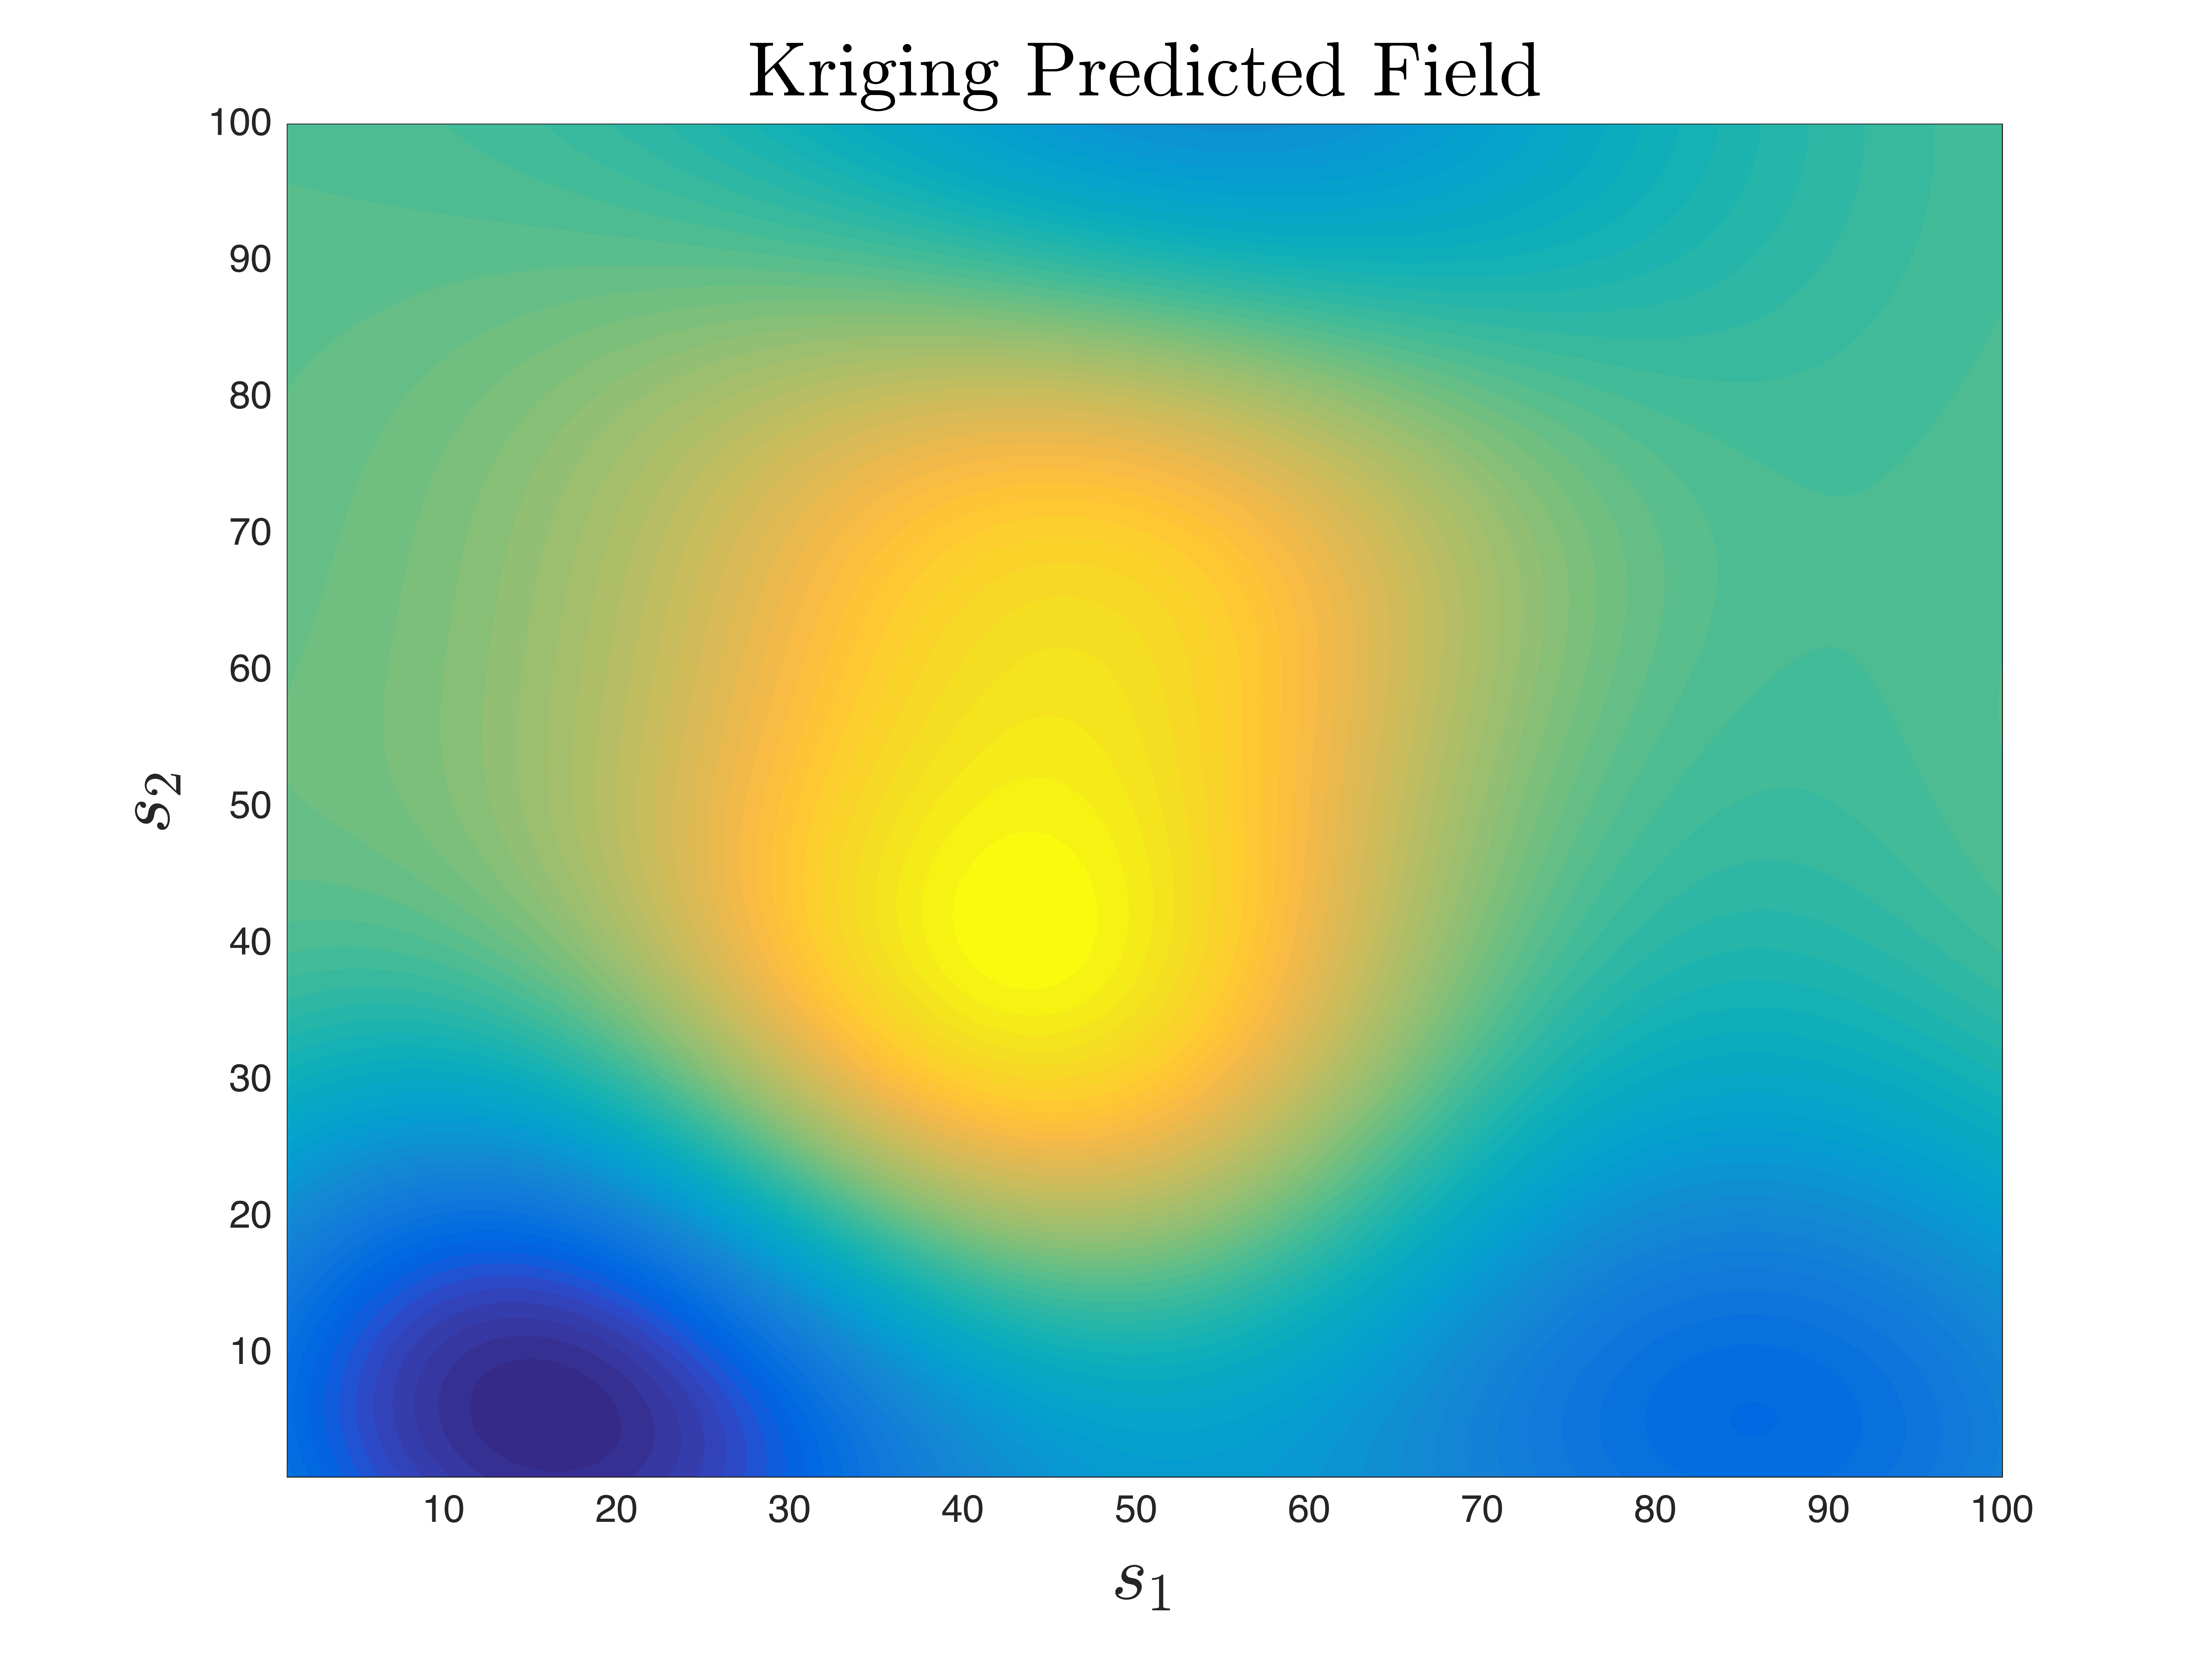
\includegraphics[width=0.8\linewidth]{figures/kriging_prediction.png}
    \ssp
    \caption{A Kriging Method predicted field generated from the samples taken of Figure \ref{fig:gen_field} at the locations marked in Figure \ref{fig:sampled_field}.}
    \label{fig:krig_field}
\end{figure}

\subsection{Variance of A Kriging Prediction} \label{sec:krigvar}
The variance of a point predicted on a target field can be calculated using byproduct terms generated along the way of calculating a Kriging prediction \cite{felus:srn}. For a predicted point $\hat{Z}(\vect{s}_0)$, using the proximity vector, $\vect{d}_0$, defined in Section \ref{sec:proxvect}, and the Kriging Weights, $\vect{\lambda}_0$ defined in Section \ref{sec:krigweights} for the predicted point, the variance of the prediction for that point is defined as:

\begin{equation}
    \text{var}\{\hat{Z}(\vect{s}_0)\} = \begin{bmatrix}\vect{d}_0 \\ 1\end{bmatrix} \begin{bmatrix}\vect{\lambda}_0^T & \mu_0 \end{bmatrix}
\end{equation}

\subsection{Procedure For Field Prediction Using The Kriging Method}
In order to predict the entirety of a target field from a finite set of $N$ observations and their respective locations, $O$, the Kriging Prediction is run at every possible unobserved vesicle in the target field. For a single iteration of collecting observations and making predictions, a covariance matrix must first be constructed, and then a the proximity vector and Kriging Weights are computed for all unobserved vesicles. The Kriging prediction formula is then used to compute the predicted value of each vesicle to predict.

\begin{algorithm}[thpb!]
\caption{Kriging Prediction of Target Field}\label{alg:krig}
\begin{algorithmic}[1]
\Procedure{KrigingPredictField}{$Z$, $O$}
\BState \emph{Generate Semi-Variogram}:
\State $\forall$ $\vect{s}_i$, $Z(\vect{s}_i)$ $\in O$:
\State \ \ \ \ $\hat{\gamma}(h) \gets \vect{s}_i$, $Z(\vect{s}_i)$\\
\BState \emph{Generate Variogram}:
\State $\gamma(h)$ fits to $\hat{\gamma}(h)$\\
\BState \emph{Construct Covariance Matrix}:
\State $\forall (\vect{s}_i,\vect{s}_j) \in O:$
\State \ \ \ \ $h_{i,j} = \|\vect{s}_i - \vect{s}_j\|_2$
\State \ \ \ \ $P_{i,j} = \gamma(h_{i,j})$\\
\State $\forall i \in [1, N]:$
\State \ \ \ \ $P_{i,N+1} = 1$
\State \ \ \ \ $P_{N+1,i} = 1$
\State $P_{N+1,N+1} = 0$\\
\BState \emph{Run Kriging Predictions For Target Field}:
\State $\forall$ $\vect{p}_i \in$ \textit{field}:
\State \ \ \ \ $\vect{d}_{i} = \begin{bmatrix} \gamma(\| \vect{s}_1 - \vect{p}_i \|_2) \dots \gamma(\| \vect{s}_N - \vect{p}_i \|_2) & 1\end{bmatrix}^T$
\State \ \ \ \ $\begin{bmatrix}
                \vect{\lambda}_{\vect{p}_i} \\
                \mu_{\vect{p}_i}
                \end{bmatrix} = \begin{bmatrix} P^{-1} & \vect{1} \\
                                    \vect{1}^T & 0 \end{bmatrix}
                                    \begin{bmatrix} 
                                    \vect{d}_{\vect{p}_i} \\
                                    1
                                    \end{bmatrix}$
\State \ \ \ \ $\hat{Z}(\vect{p}_i) = \begin{bmatrix} Z(\vect{s}_1) \dots Z(\vect{s}_N) \end{bmatrix} \lambda_{\vect{p}_i}$
\State \ \ \ \ $\text{var}\{\hat{Z}(\vect{p}_i)\} = \begin{bmatrix}\vect{d}_i \\ 1\end{bmatrix} \begin{bmatrix}\vect{\lambda}_{\vect{p}_i}^T & \mu_{\vect{p}_i} \end{bmatrix}$
\EndProcedure
\end{algorithmic}
\end{algorithm}

When Algorithm \ref{alg:krig} is run on the target field from Figure \ref{fig:gen_field}, for the samples taken in Figure \ref{fig:sampled_field}, a prediction of the entire field can be generated, as seen in Figure \ref{fig:krig_field}.